\noindent \textred{4.} 
\textbf{(5 points)} \textit{Implementing back-propagation in Python from scratch}. Open the (incomplete) Jupyter notebook provided as an attachment to this homework in Google Colab (or other Python IDE of your choice) and complete the missing items. In the second demo, we worked with autodiff. Autodiff enables us to implicitly store how to calculate the gradient when we call backward. We implemented some basic operations (addition, multiplication, power, and ReLU). In this homework problem, you will implement backprop for more complicated operations directly. Instead of using autodiff, you will manually compute the gradient of the loss function for each parameter.
\\ \\
\noindent \myAnswer{
The whole PDF exported from Jupyter notebook is attached at the end, in which the back-propagation was implemented in pure NumPy. \\
After training for 1 epoch, the network achieved $\sim 70\%$ accuracy on the test set. \\
After 3 epochs, the testing accuracy didn't improve (even decreased a little bit, probably due to over-fitting).
}
\begin{figure}[!h]
    \centering
    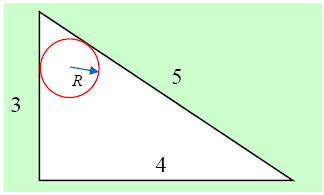
\includegraphics[width=\linewidth]{HWs//HW1//figures/4.png}
\end{figure}